\documentclass[11pt]{article}   	
\usepackage{geometry}
\geometry{letterpaper}                   		% ... or a4paper or a5paper or ... 
\usepackage{graphicx}	
\graphicspath{{images/}}			% Use pdf, png, jpg, or eps§ with pdflatex; use eps in DVI mode
\usepackage{float}							% TeX will automatically convert eps --> pdf in pdflatex
\usepackage{listings}								 	
\usepackage{amssymb}
\usepackage[T1]{fontenc}
\usepackage[framed,numbered,autolinebreaks,useliterate]{mcode}

\title{MAT 128B  Project}
\author{Xinke Yu}
\date{}							% Activate to display a given date or no date

\begin{document}
\maketitle

\section{An introduction to fractuals}
The \textbf{orbit}  of $z_0$ under $\phi$ is the sequence generated by repeated application of the mapping $\phi (z)$ with initial value $z_0$.\\
The \textbf{filled Julia set} of a polynomial function $\phi(z)$ is the set of points $z_0$ for which the orbit remains bounded.\\
The \textbf{Julia set} is the boundary of a filled Julia set.\\
The \textbf{Mandelbrot set} is the set of points $c$ such that $\phi(z) = z^2 + c$ does not diverge when starting with $z_0 = 0$.\\
\begin{figure}[!hbp]
  \centering
  \begin{minipage}[b]{0.45\textwidth}
    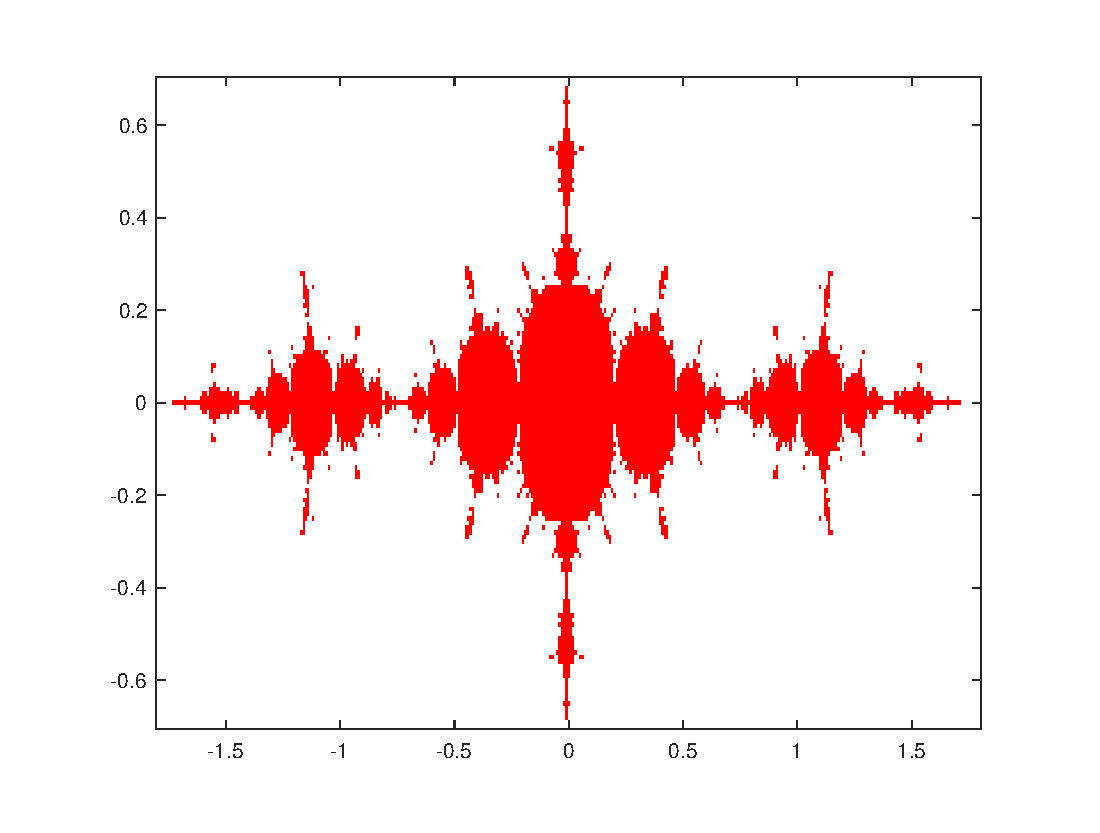
\includegraphics[width=\textwidth]{JuliaSet_fig413.eps}
    \caption{$\phi(z)=z^2-1.25$}
  \end{minipage}
  \hfill
  \begin{minipage}[b]{0.45\textwidth}
    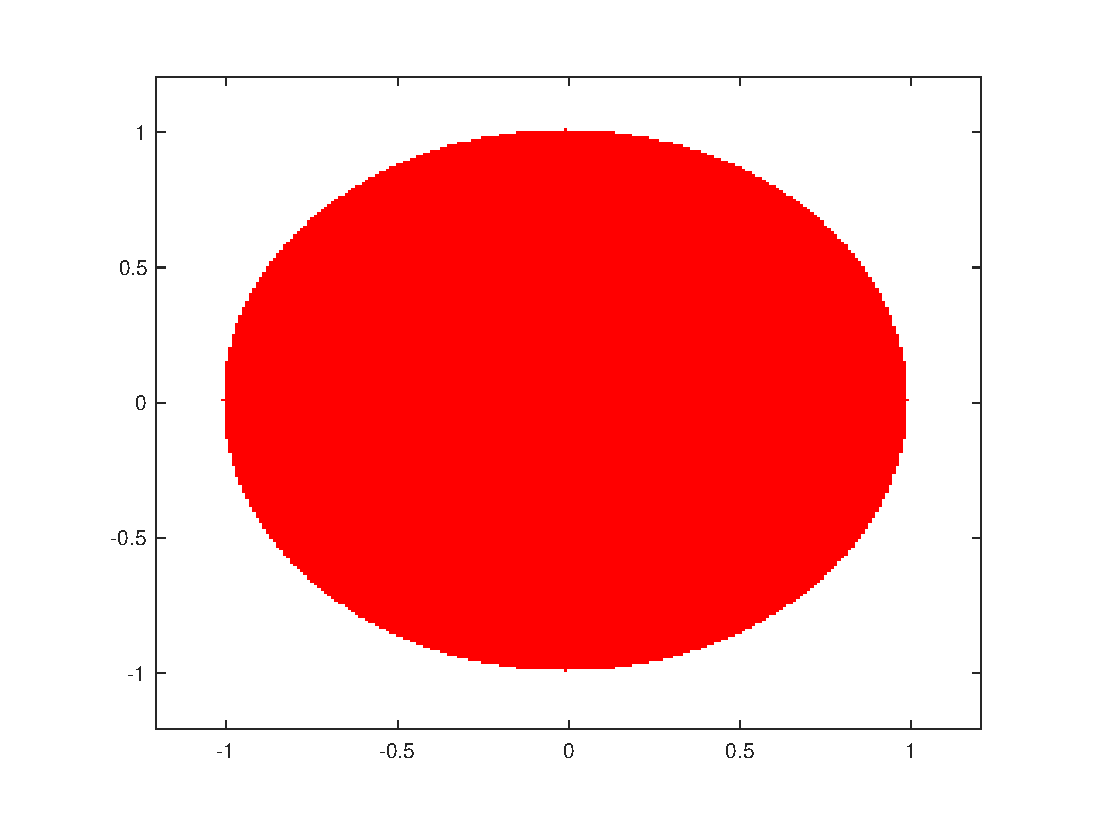
\includegraphics[width=\textwidth]{juliaSet_z2.eps}
    \caption{$\phi(z)=z^2$}
  \end{minipage}
\end{figure}


\section{Generate other examples changing the value of c}
When $z_0$ changes, $\phi(z)$ will either converge or diverge depending on the value of c. However, for any $c$ value, the iteration method diverges when $|z|> 2$.\\
The filled Julia sets for different values of c:\\
\begin{figure}[H]
  \centering
  \begin{minipage}[b]{0.45\textwidth}
    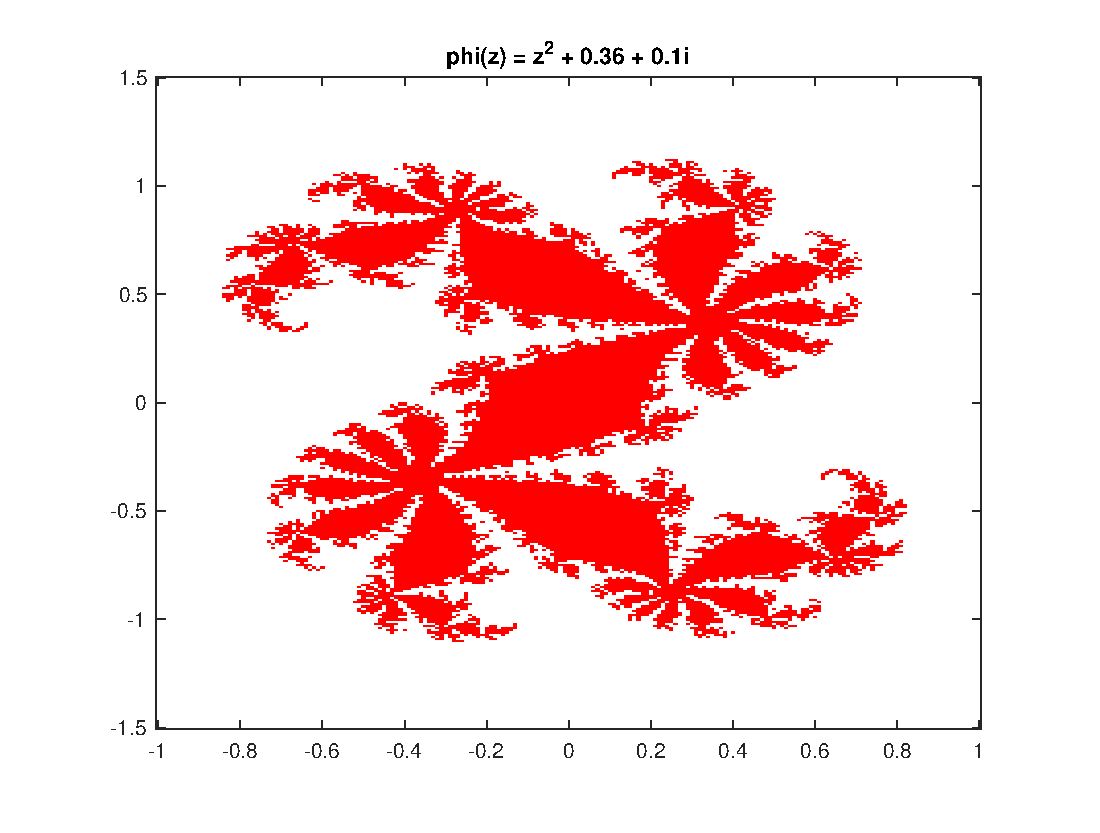
\includegraphics[width=\textwidth]{part2func1.eps}
    \caption{$c = 0.36 + 0.1i$}
  \end{minipage}
  \hfill
  \begin{minipage}[b]{0.45\textwidth}
    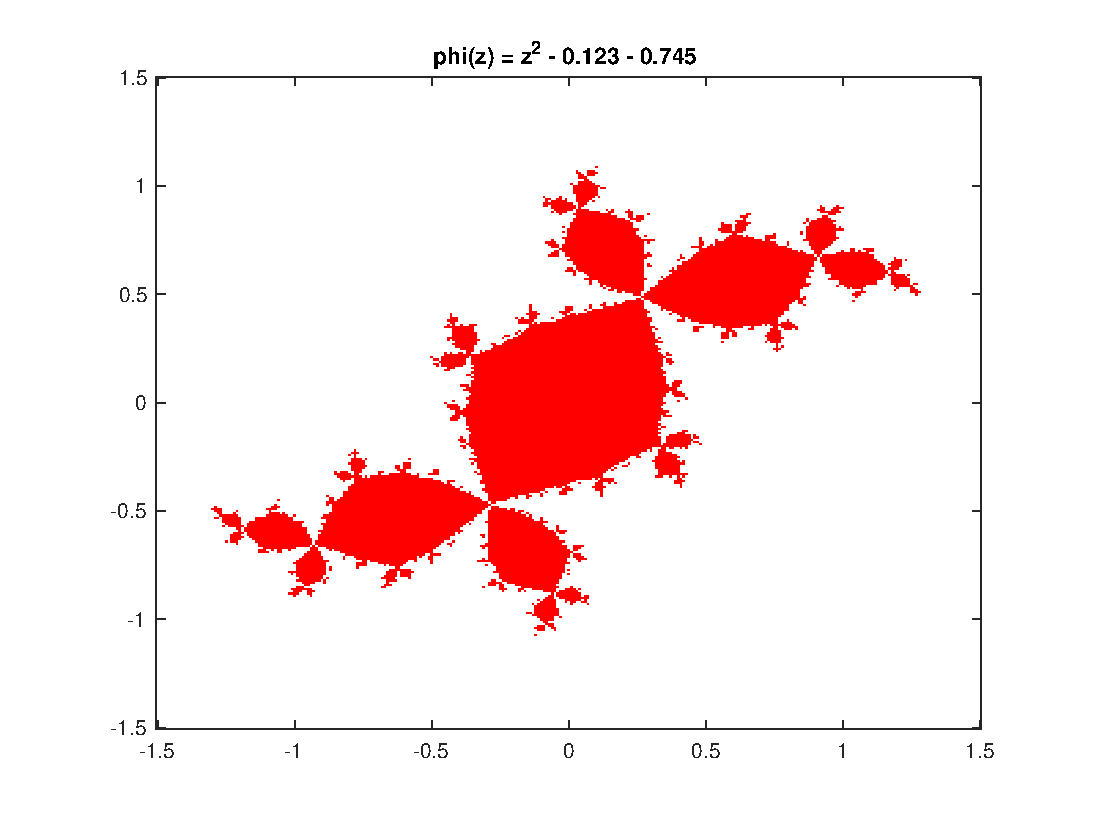
\includegraphics[width=\textwidth]{part2func2.eps}
    \caption{$c = -0.123 - 0.745i$}
  \end{minipage}
   \end{figure}
   
   \begin{figure}[!h]
  \begin{minipage}[b]{0.45\textwidth}
    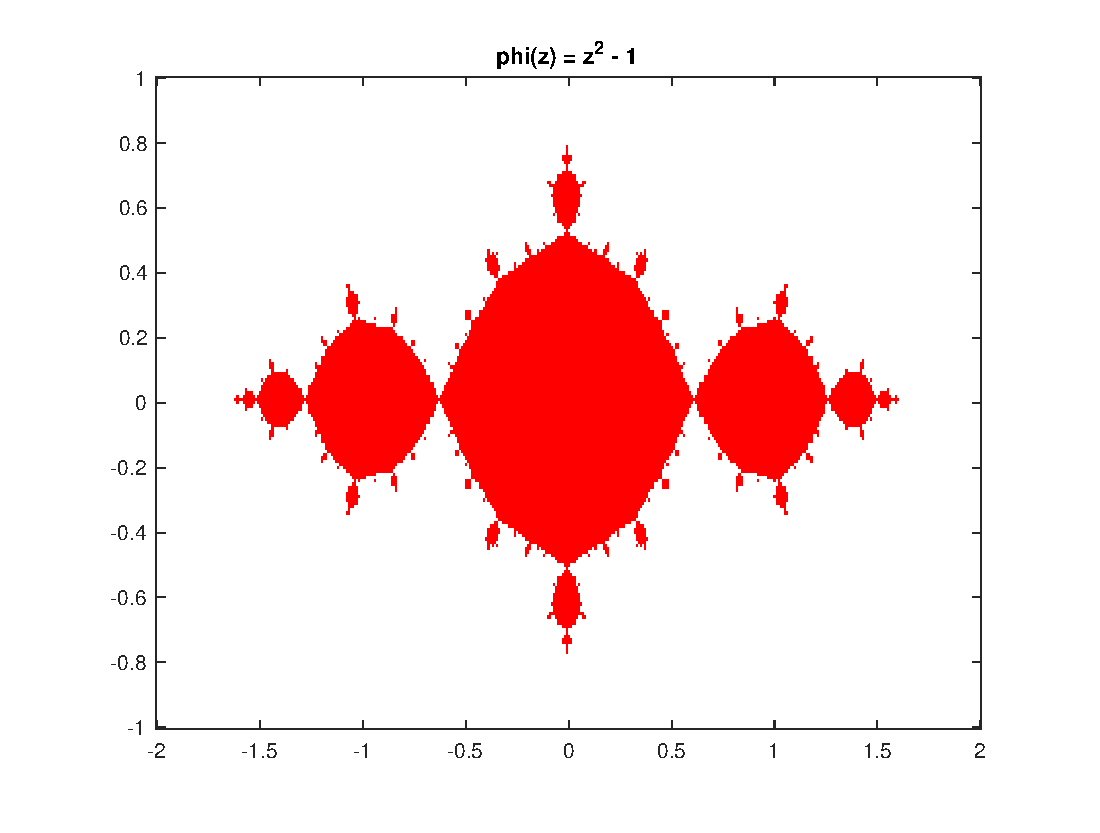
\includegraphics[width=\textwidth]{part2func5.eps}
    \caption{$c = -1$}
  \end{minipage}
  \hfill
  \begin{minipage}[b]{0.45\textwidth}
    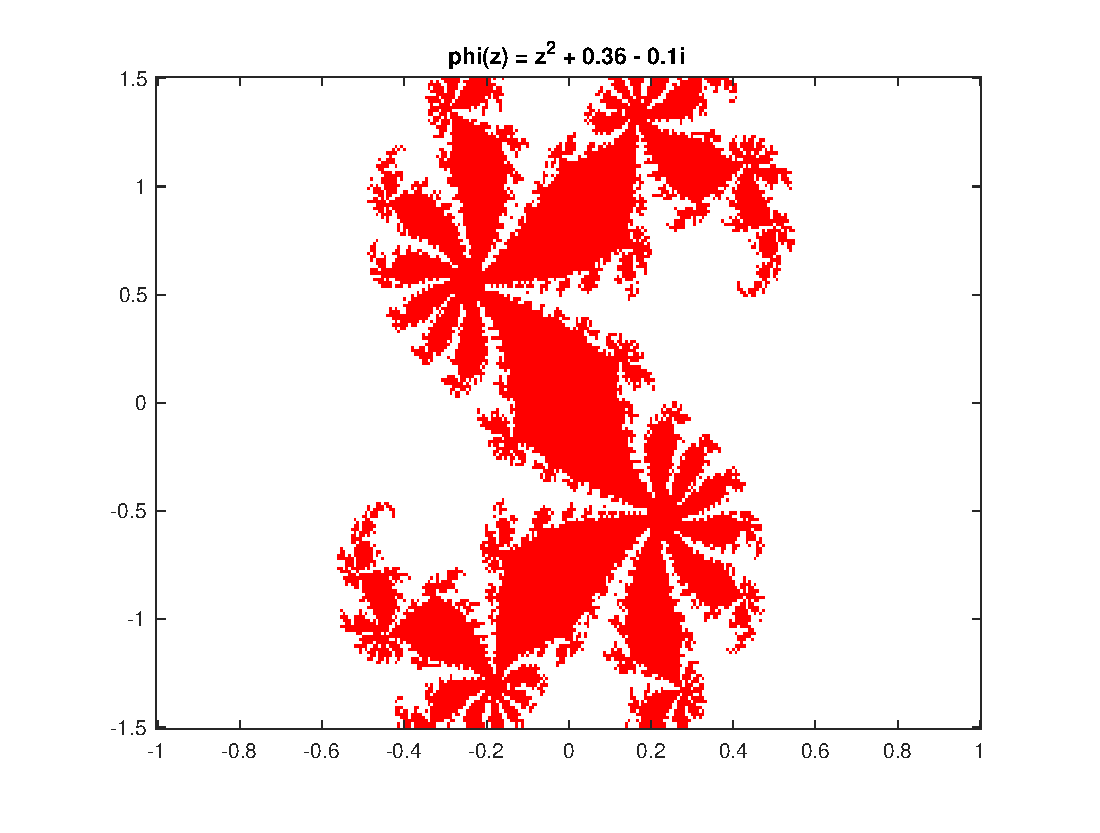
\includegraphics[width=\textwidth]{part2func6.eps}
    \caption{$c = -i$}
  \end{minipage}

\end{figure}

\section{Constructing the Julia Set}
$$z_{n+1} = z_n^2 +c\rightarrow \textrm{ the inverse is: }z_{n+1} = \pm\sqrt{z_{n}-c}$$\\
Let $z_{n+1} = x_{n+1} + iy_{n+1}, z_n = x_n + iy_n$, and $c = x_0 + iy_0$.\\
Then $$x_{n+1}+iy_{n+1} = \pm\sqrt{x_n+iy_n-x_0-iy_0} = \pm\sqrt{(x_n-x_0)-i(y_n-y_0)} $$
Let $(x_n-x_0)-i(y_n-y_0) = re^{i\theta}$.\\
Then $$x_{n+1}+iy_{n+1} =\pm \sqrt{r}e^{i\frac{\theta}{2}} = \pm\sqrt{r}(\cos(\frac{\theta}{2})+i\sin(\frac{\theta}{2}))$$,\\
where $$r = \sqrt{(x_n-x_0)^2 + (y_n-y_0)^2},$$$$ \theta = \tan^{-1}{\frac{y_n-y_0}{x_n-x_0}}\textrm{  (add $\pi$ to $\theta$ if $x_n-x_0 < 0$)}$$
Therefore, $$x_{n+1} = \pm\sqrt{r}\cos(\frac{\theta}{2}) \textrm{, }y_{n+1} = \pm\sqrt{r}\sin(\frac{\theta}{2})$$
Keep applying these two iterations ($x_n$ generates the real part and $y_n$ generates the imaginary part) while randomly choosing the branches for the square root will generate the Julia set.\\
\\
\textbf{Matlab Code}:
\begin{lstlisting}
function [] = constructJuliaSet(x,y)
%construct the Julia set for c = x+iy
numofIt = 100; %number of iterations
rangeUpper = 41; %determines the number of z_n's
increment = 4/(rangeUpper-1);
c = x+1i*y;

figure %for plotting
hold on
for i = 1: rangeUpper %choose initial values from -2 to 2
    x_co = -2 + (rangeUpper-1)*increment; %real part
    for j = 1: rangeUpper 
       y_co = -2 + (rangeUpper-1)*increment; %imaginary part 
       rnew = sqrt(sqrt((x_co-x)^2+(y_co-y)^2));
       theta = atan((y_co-y)/(x_co-x));
       if(x_co-x)<0
           theta = theta + pi;
       end
       xnew = rnew * cos(theta/2);
       ynew = rnew * sin(theta/2);
       k = 0;

       while k <= numofIt
           k = k + 1;
           randNum = round(rand()); %random number that determines which branch to pursue
           if (randNum == 1)%positive branch
              rnew = sqrt(sqrt((xnew-x)^2+(ynew-y)^2)); %values for the next iteration
              theta = atan((ynew-y)/(xnew-x));
              if(xnew-x)<0
                theta = theta + pi;
              end
              xnew = rnew * cos(theta/2);
              ynew = rnew * sin(theta/2);
           else %randNum == 0, negative branch
              rnew = sqrt(sqrt((xnew-x)^2+(ynew-y)^2)); %essentially the same as above, just negate final value
              theta = atan((ynew-y)/(xnew-x));
              if(xnew-x)<0
                theta = theta + pi;
              end
              xnew = -rnew * cos(theta/2);
              ynew = -rnew * sin(theta/2);
           end
       end
       plot(xnew, ynew, '.');
    end
    
end

end

\end{lstlisting}


\end{document}  